% Activate the following line by filling in the right side. If for example the name of the root file is Main.tex, write
% "...root = Main.tex" if the chapter file is in the same directory, and "...root = ../Main.tex" if the chapter is in a subdirectory.
 
%!TEX root =  ../Thesis.tex

\chapter[Background Estimation]{Background Estimation}

Once the background has been reduced as much as practical using the trigger and kinematic cuts,
a reliable estimate of the shape and size of the remaining background is critical to optimizing
the exclusion limits.  In particular, since the reconstructed mass peak of the $b$-jets is so
broad in signal, a mis-estimation of the background shape can lead to systematic errors that
could wash out any possible signal (or worse, be mistaken for a signal where there is none).  

At the same time, the backgrounds in this analysis are challenging to estimate, either in Monte
Carlo or using data-driven methods.  Therefore, much of the work of this analysis is dedicated
to validating the background estimation and providing uncertainties for especially the shape 
of the background.  

\section{Background Estimation Strategy}
\label{sec:background_strategy}
As QCD is the dominant background in this analysis, it is important to understand
what flavors of QCD jets compose the population of events that survive the cut
chain.  In order to do this, we apply the trigger and all cuts up to (but not including)
requiring a third $b$-tagged jet in the event.

 The signal and background are then split into 3 exclusive regions, defined as follows:
\begin{itemize}
    \item \textit{bbb}: one or more jets (in addition to the two triple-tagged jets) passing a tight (60\% working point)
 MV1 cut–-in effect, the full signal selection criteria
    \item \textit{bbloose}: events failing the bbb classification but which have one or more jets passing a loose (80\%
 working point) MV1 cut
    \item \textit{bbanti}: events that have no jets passing an 80\% MV1 cut-–effectively a veto on the presence of any
 $b$-tagged jets other than those firing the trigger
\end{itemize}



\section{Background Estimation Method Based on Exponential Background Model and Sideband Fitting}
The background consists almost exclusively of QCD with 2 or more real $b$-jets, which 
fortunately has a $m_{bb}$ spectrum that does not have any peaks or other difficult
structure above about 350 GeV.  Below that mass, the trigger turn-on curve becomes
a major feature of the spectrum.  Above that mass, there
is a smoothly falling distribution that we fit primarily with a decaying exponential.

In a few words, the background fit strategy proceeds in the following way:
\begin{itemize}
    \item Start with a mass point
    \item Apply a mass-point-specific rotation based on the the eigenvectors of 
    the signal MC, as calculated using $m_{bb}$, $p_{T}^1$ and $p_T^2$; call 
    the components of this rotated basis $m_{bb}'$, $p_T^{1'}$ and $p_T^{2'}$
    \item Apply cuts to $p_T^{1'}$ and $p_T^{2'}$, and use $m_{bb}^{'}$ as the final 
    discriminating variable 
%    \item Using the signal MC as a guide, select a window in $m_{bb}$ that encloses the
%signal peak, along with as much of the mass sideband (on either side) as possible
    \item Fit an exponential function to the $m_{bb}^{'}$ distribution, allowing each of the 
tag regions (\textit{bbb}, \textit{bbloose}, \textit{bbanti}) to float relative to each other
 as well as keeping the 3, 4, and 5+ jet categories separate
    \item As part of the limit-setting procedure, use the fit result for the 
    background along with signal shapes taken from MC to extract the 
signal cross section that can be excluded at a 95\% confidence level
    \item Repeat for the next mass point
\end{itemize}

Although we have signal MC with $m_A$ values as low as 250 GeV, this fit strategy only
begins to work above 400 GeV, because of the trigger turn-on curve.  The fit window
used is [340,900] GeV for all signal mass points.

While the analysis was in development, it was blinded to avoid bias.  This was done 
by removing \textit{bbb} events from the data, and replacing them with a sample of
events with the same normalization drawn from the \textit{bbanti} distribution
in data.  For the final search, the \textit{bbb} events were swapped back in.



%\section{Turn-On Curve Modeling}
%Although the lowest part of the $m_{bb}$ distribution (below 300 GeV) is not part of the search regime,
%because of the rapidly changing background, including it in the background model helps
%improve the overall fit by allowing for a slightly fewer events at moderately low
%$m_{bb}$ (between about 300 and 400 GeV) than an exponential alone would predict.
%The turn-on is fit with a logistic function of the form

%\begin{equation}
%f(m_{bb}) = N\frac{1}{1+e^{-c(m_{bb}+d)}}
%\end{equation}

%In this equation, N controls the overall normalization, $c$ governs the steepness
%of the turn-on curve, and $d$ is the horizontal offset.

%\textbf{once we confirm this (or something like it) as the final fit model,
%add a plot showing how this function changes with c/d and the composite
%model of exponential times logistic}


\section{Eigenvector Rotation}
\textbf{If Tim's eigen-analysis is validated and used, a description of that method goes here}

\begin{itemize}
    \item for high-mass points, we have trouble when FSR is bad (but it isn't always bad)
    \item FSR is worst when jets are low-pT--suggests a cut or categorization based
    on pT of the jets
    \item However, simple cut can sculpt background b/c of correlations btwn pT1, pT2, mbb,
    and it also reduces background to rates too low to model well
    \item use signal MC to identify eigenvectors based on pT1, pT2 and mbb, transform
    into this basis 
    \item Place cuts on pT1' and pt2'
    \item Use $mbb'$ as the discriminating variable, proceed to fit with exponential
    \item Impact on final sensitivity in the results section
\end{itemize}

Once the events have been categorized based on $b$-tag status and the number of jets in the
events, but before doing the final fit, we apply a change of variables based on the jet
$p_T$ values and $m_{bb}$ in each event and a kinematic cut.  Together these analysis 
steps effectively allow for a discriminating variable, which we call $m_{bb}'$, that
separates signal and background better than ordinary $m_{bb}$.  Once these steps have
been applied, the result is an analysis that is 15-50\% more sensitive
than if no transformation were applied.  This section will 
outline this procedure and its rationale.  

The motivation for this strategy has its origins in trying to control the effect of
FSR on the analysis sensitivity.  At high $m_A$, the jets from the Higgs (and also 
the associated $b$-quark) have large $p_T$, which they then tend to radiate away 
as FSR.  This causes the $m_{bb}$ peak to smear out and be more difficult to 
distinguish from background than in the lower-$m_A$ cases.  However, since FSR
occurs stochastically on an event-by-event basis, a subset of the signal events
will have little or no FSR and will reconstruct to $m_A$--if these events 
can be isolated from the others, they offer a chance to improve the sensitivity
via the improved mass resolution and signal-to-background ratio. 

A simple strategy might be to apply a cut to the $p_T$ of the leading and/or 
second jet in the event, and only accept events where the $p_T$ is above some
threshold optimized by comparing signal MC to \textit{bbanti} data.  
That would isolate events with poor mass resolution (i.e. lots of FSR) from
those with little FSR and better reconstruction properties.  However, since
there is a correlation between $p_T^1$, $p_T^2$ and $m_{bb}$, a cut like
this ends up sculpting the background as well.  In addition, the $p_T^1$ and
$p_T^2$ cut thresholds that looked best on signal MC are ``too good'' on 
background-dominated \textit{bbanti} events and there is no background
above a certain $m_{bb}$ value.  That makes modeling the background extremely 
difficult, and any fit difficult to validate.  

Adding a change of basis before the $p_T$ cuts turns out to offer the advantage
of better signal/background separation without the cost of making the background
difficult to model.  The basis change is a rotation away from the $p_T^1$, 
$p_T^2$, $m_{bb}$ basis into what we call the $p_T^{1'}$, $p_T^{2'}$, $m_{bb}^{'}$
basis, where $p_T^{1'}$, $p_T^{2'}$, $m_{bb}^{'}$ are the eigenvectors of 
a matrix built out of $p_T^1$, $p_T^2$, and $m_{bb}$.  The leading eigenvector 
\footnote{the leading eigenvector is defined as the eigenvector with the largest
associated eigenvalue}, which we call $m_{bb}^{'}$, is an admixture of 
$p_T^1$, $p_T^2$, and $m_{bb}$, the exact blend of which varies by signal mass
point.  The relative contributions of $p_T^1$, $p_T^2$, and $m_{bb}$ to the $m_{bb}^{'}$
leading eigenvector can be seen in Table~\ref{tab:eigenvector_elements}.


\begin{table}
    \caption{The major axis eigenvector elements, and their squares.  The
    transformation into the eigenbasis makes use of the raw elements, but the
    squares of the elements sum to 1.0 and can provide some physical intuition
    for the relative contributions of $p_T^1$, $p_T^2$ and $m_{bb}$. \label{tab:eigenvector_elements}}
    \begin{tabular}{ c c c c c c c } \hline \hline
        $m_A$ & $m_{bb}$ & $p_T^1$ & $p_T^2$ & $m_{bb}^2$ & $(p_T^{1})^2$ & $(p_T^2)^2$ \\ \hline
        450 & 0.87 & 0.35 & 0.35 & 0.76 & 0.12 & 0.12 \\
        500 & 0.84 & 0.38 & 0.39 & 0.71 & 0.14 & 0.15 \\
        550 & 0.80 & 0.40 & 0.46 & 0.64 & 0.16 & 0.21 \\
        600 & 0.78 & 0.41 & 0.47 & 0.61 & 0.17 & 0.22 \\
        650 & 0.72 & 0.46 & 0.52 & 0.52 & 0.21 & 0.27 \\
        700 & 0.71 & 0.47 & 0.54 & 0.50 & 0.22 & 0.29 \\
        800 & 0.67 & 0.50 & 0.55 & 0.45 & 0.25 & 0.30 \\ 
        \hline
    \end{tabular}
\end{table} 

As Table~\ref{tab:eigenvector_elements} shows, the largest component of
$m_{bb}^{'}$ comes from $m_{bb}$, regardless of the mass point.  However,
for higher $m_A$ values, there is the clear trend that $p_T^1$ and $p_T^2$
components become larger, meaning that the $p_T$s of the jets becomes 
more important as $m_A$ grows.  This is consistent with the original 
physical hypothesis behind this strategy, which is to isolate and remove
high-FSR events, of which there are more for the larger values of $m_A$. 
The effect of this transformation on 800 GeV signal and background-dominated
data can be seen in Figure ~\ref{fig:transformed_vars}.  These figures show
the difference in the mass and $p_T$ distributions before and after the transformation,
with the mass distribution in particular being pushed to lower values
in the background distribution while the signal mass maintains a similar shape.  
This background reshaping affects the signal to background ratio in the 
neighborhood of the signal peak; before the rotation,
a line drawn at the nominal $m_A$ value (800 GeV) shows that there is still
significant background remaining, but after the rotation the signal is virtually
unchanged while the background has been shifted lower.  An examination of the
$p_T$ variables shows that before the transformation, the signal and background
shapes are different; however, after the rotation, the signal and background
shapes are virtually identical.  This reinforces the hypothesis that projecting
onto the major axis is effectively concentrating all of the discriminating 
power in $m_{bb}$, $p_T^1$, and $p_T^2$ together into the single $m_{bb}^{'}$
variable.  

\begin{figure}[hbt]
\includegraphics[width=\linewidth]{BackgroundEstimation/images/vars_before.pdf}
\includegraphics[width=0.45\linewidth]{BackgroundEstimation/images/vars_after.pdf}
\caption{variables before and after the rotation\label{fig:ttbar_mbb}}
\end{figure}

However, there is one more step that optimizes the signal to background
discrimination further, which is placing cuts on $p_T^{1'}$ and $p_T^{2'}$.
If we require that $p_T^{1'}>-10$ GeV, and $p_T^{2'}>-50$ GeV, it 
excludes a region of $m_{bb}^{'}$ phase space where the modeling is difficult
and little sensitivity is gained.  






\section{Mathematical Modeling of Background Shape}
\subsection{Selection of Exponential Function}
Once the rotation and cuts have been applied, the data is fed into an 
unbinned maximum likelihood fit for mathematical modeling.  The fitting
of both signal and background is done in RooFit.  There are a number 
of candidate functions for the background fit, which can be evaluated
both on their goodness-of-fit (as measured by a metric like $\chi^2/DOF$)
and their ease of convergence.

In brief, the functions given consideration include the following:
\begin{itemize}
    \item \textbf{Bernstein Polynomial}
    \item \textbf{Power Decay Series}
    \item \textbf{Decaying Exponential with 1 parameter}
    \item \textbf{Decaying Exponential with 2 parameters}
\end{itemize}

\subsubsection{Bernstein Polynomials}
The Bernstein polynomials are a family of polynomials that are characterized
particularly by their attractive feature of being positive-definite, or never
predicting a negative value for a PDF composed of them.  However, we find
that it takes a high degree of polynomial (5 parameters or more) to fit the
background over the full mass range (340,900 GeV), and a polynomial with a 
degree this high struggles (and often fails) to converge.  Moreover, a
drawback of high-degree polynomials is their capability to ``wiggle'' and
potentially absorb a signal within the background model.

\subsubsection{Power Decay Series}
A power decay series of the form $\frac{a}{x} + \frac{b}{x^3} + \frac{c}{x^5} + ...$
is another possibility; if all the powers of $x$ in the denominators are
odd, this series cannot wiggle like the Bernstein polynomials.  However,
a simple series with a few terms does not fit the background shape well 
over the full mass range, and when many terms are added to the series then
the fit struggles to find a global maximum of the likelihood function, leading
to non-convergence.

\subsubsection{Decaying Exponential with 1 Parameter}
Like a decaying power series, a decaying exponential function is monotonically
decreasing; however, unlike a power series, an exponential with a single
parameter (i.e. a model of the form $f(x)=e^{-x/\tau}$) provides 
a relatively good fit to the background distribution in most tag and jet
categories, with $\chi^2/DOF$ values below 2 for all \textit{bbb} and \textit{bbloose}
distributions \footnote{the \textit{bbanti} distributions prove harder to
fit with a 1-parameter exponential, with $\chi^/DOF$ values between 2.8 and 3.9}.
Additionally, the simplicity of a 1-parameter exponential means that the
fits converge quickly and reliably over the full mass range.

\subsubsection{Decaying Exponential with 2 Parameters}
A decaying exponential with two parameters (i.e. a model of the form $f(x)=e^{-x/\tau+\omega x^2}$)
has the same nice features of a single-parameter exponential (simple functional
form, easy convergence, no possibility of signal-spoofing wiggles) while offering
more flexibility than the 1-parameter exponential.  The $\chi^2/DOF$ and pulls
for the 2-parameter exponential fits reflect this flexibility to better
fit the data, every jet/tag category has a fit that is as good or better
for the 2-parameter exponential as for the 1-parameter exponential.  In 
particular, the \textit{bbanti} categories that have higher $\chi^2/DOF$ values
in the 1-parameter fit show $\chi^2/DOF$ results of 1.0-1.2 with the 2-parameter fits. 



\subsection{Background Shape and Spurious Signal}
\cite{spurious_signal}












\subsection{Non-QCD Backgrounds}
\label{sec:non_qcd_bkgs}

\subsubsection{All-Hadronic $t\bar{t}$ Background}
When $t\bar{t}$ decays all-hadronically, it can create events with several high-$p_T$
jets and 2 or more $b$-tagged jets (where the $b$-tags come from both real $b$-quarks
and from mistagged light flavor).  We anticipate that, because it has a production
cross section that is much smaller than QCD, $t\bar{t}$ will not be a major background.
We confirm this assumption in MC by using the all-hadronic $t\bar{t}$ sample summarized
in Table~\ref{tab:ttbar_params}.


We find that in MC, all-hadronic $t\bar{t}$ has an efficiency of 7.5\% after
the EF\_2j35\_loose\_j145\_j35\_a4tchad trigger, and approximately 2\% efficiency
in the offline cuts relative to the trigger.  Estimating the $t\bar{t}$ cross section
as 165 pb, and a 44\% branching ratio in the all-hadronic decay channel, this gives
a 0.11 pb $t\bar{t}$ cross section expected after the trigger and offline cuts.  In the
full 2012 dataset, this amounts to about 2400 events.  While
this is not a negligible cross section compared to the signal, it is more than an
order of magnitude smaller than the QCD background.

In addition to checking the magnitude of the $t\bar{t}$ background, we check the shape
for any shape differences in the $m_{bb}$ distribution depending on the tag status of the
third jet, and do not find any major discrepancies that point toward $t\bar{t}$ as a
potential peaking background in the signal region. The $m_{bb}$ distributions in the
bbb, bbloose and bbanti bins for the all-hadronic $t\bar{t}$ can be found in Figure
~\ref{fig:ttbar_mbb}.




\begin{figure}[hbt]
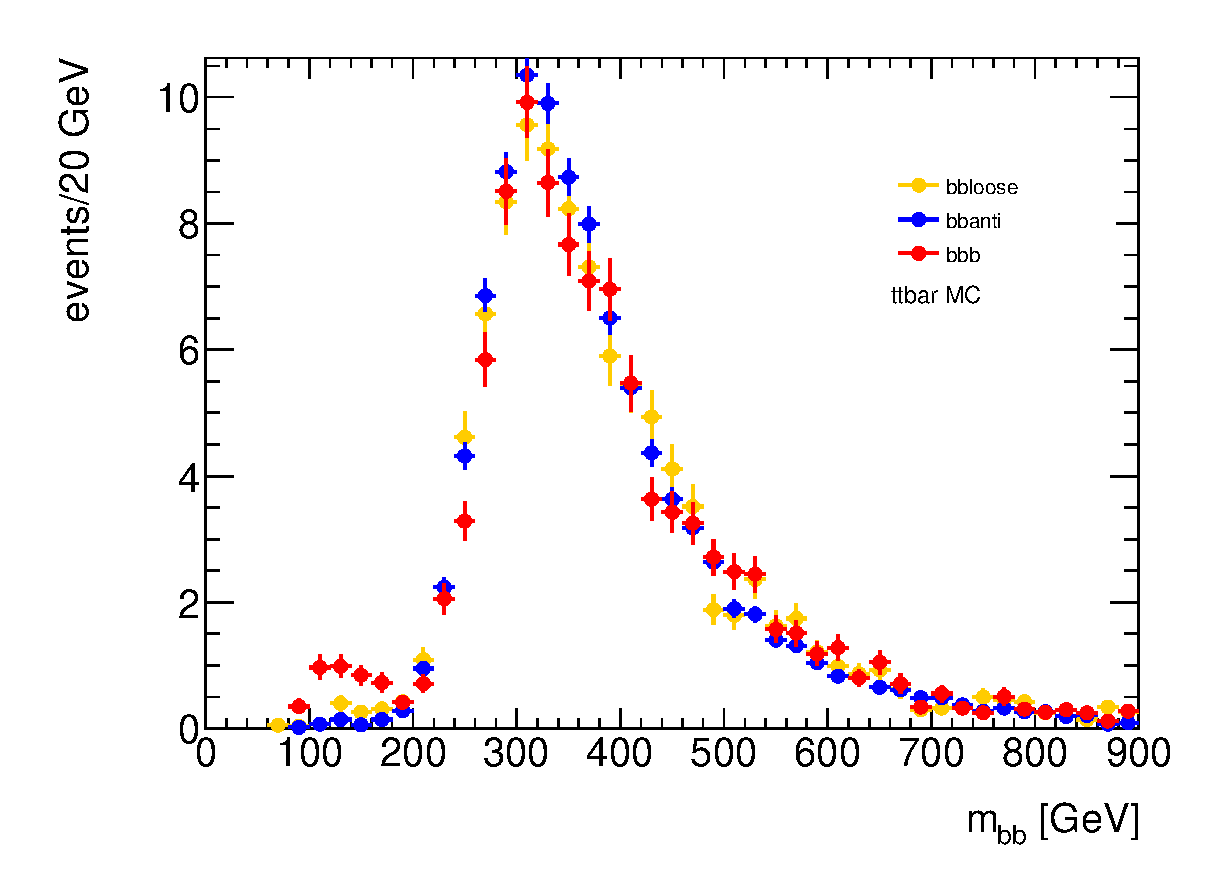
\includegraphics[width=0.45\linewidth]{BackgroundEstimation/images/mbb_compare_bbb_bbloose_bbanti_ttbar.eps}
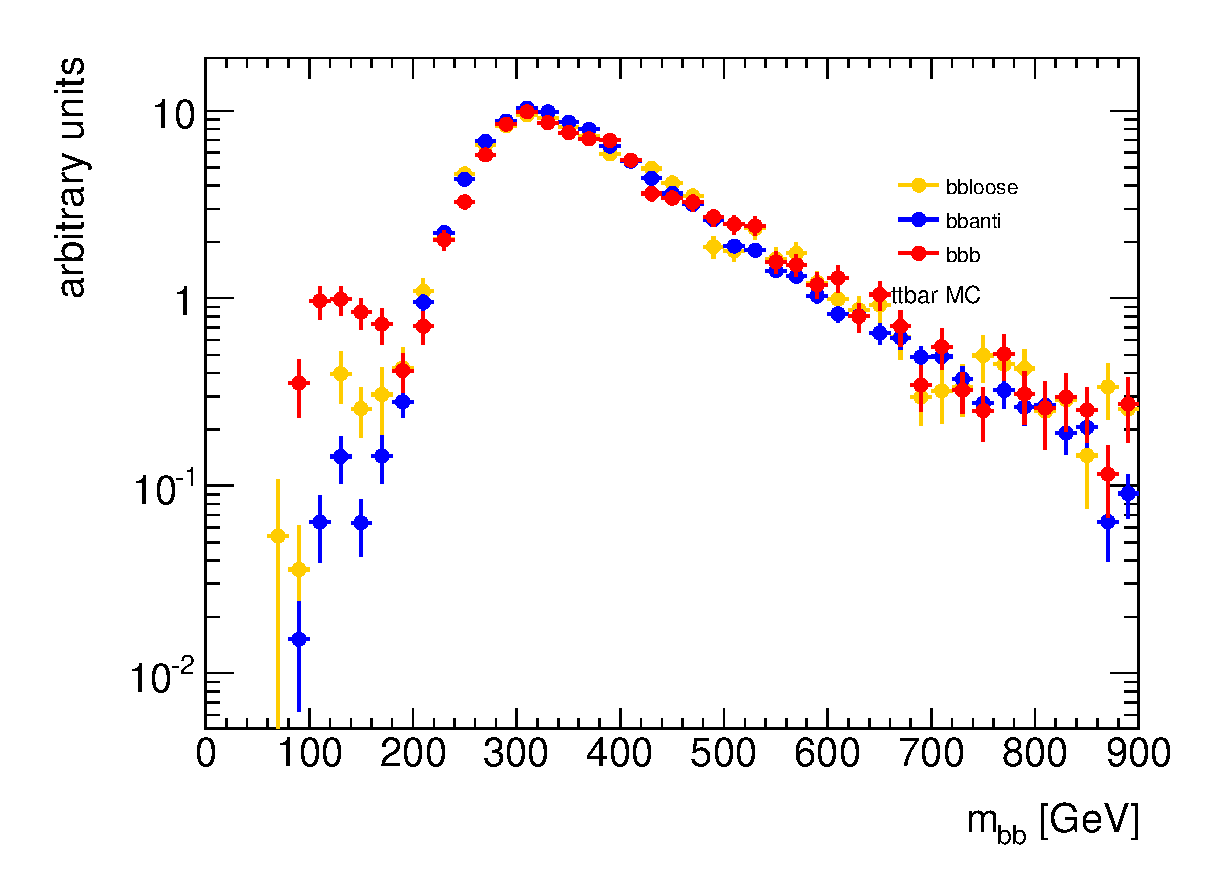
\includegraphics[width=0.45\linewidth]{BackgroundEstimation/images/mbb_compare_bbb_bbloose_bbanti_ttbar_logy.eps}
\caption{The $m_{bb}$ distributions for all-hadronic $t\bar{t}$ MC after the trigger and all offline cuts are applied (linear Y axis on the left, logarithmic scale on the right).  In addition to the overall cross-section, we also want to probe any shape differences that arise when the tag status changes on the third jet in the event.  No significant shape differences are seen.}
\label{fig:ttbar_mbb}
\end{figure}

















